\documentclass[letterpaper,10pt]{article}

\usepackage{enumitem}
\usepackage{titling}
\usepackage{listings,listings-rust}
\usepackage{url}
\usepackage{soul}
\usepackage{hyperref}
\usepackage{setspace}
\usepackage{subfig}
\usepackage{sectsty}
\usepackage{pdfpages}
\usepackage{colortbl}
\usepackage{multirow}
\usepackage{multicol}
\usepackage{relsize}
\usepackage{amsmath}
\usepackage{wasysym}
\usepackage{fancyvrb}
\usepackage[yyyymmdd]{datetime}
\usepackage{amsmath,amssymb,amsthm,graphicx,xspace}
\usepackage[titlenotnumbered,noend,noline]{algorithm2e}
\usepackage[compact]{titlesec}
\usepackage{XCharter}
\usepackage[T1]{fontenc}
\usepackage[scaled]{beramono}
\usepackage[normalem]{ulem}
\usepackage{booktabs}
\usepackage{tikz}
\usetikzlibrary{arrows.meta,automata,shapes,trees,matrix,chains,scopes,positioning,calc,decorations.pathreplacing}
\tikzstyle{block} = [rectangle, draw, fill=blue!20, 
    text width=2.5em, text centered, rounded corners, minimum height=2em]
\tikzstyle{bw} = [rectangle, draw, fill=blue!20, 
    text width=4em, text centered, rounded corners, minimum height=2em]

\definecolor{namerow}{cmyk}{.40,.40,.40,.40}
\definecolor{namecol}{cmyk}{.40,.40,.40,.40}
\renewcommand{\dateseparator}{-}

\let\LaTeXtitle\title
\renewcommand{\title}[1]{\LaTeXtitle{\textsf{#1}}}

\lstset{basicstyle=\footnotesize\ttfamily,breaklines=true}

\newcommand{\CPP}{C\nolinebreak\hspace{-.05em}\raisebox{.4ex}{\tiny\bf +}\nolinebreak\hspace{-.10em}\raisebox{.4ex}{\tiny\bf +}}
\def\CPP{{C\nolinebreak[4]\hspace{-.05em}\raisebox{.4ex}{\tiny\bf ++}}}

\newcommand{\handout}[5]{
  \noindent
  \begin{center}
  \framebox{
    \vbox{
      \hbox to 5.78in { {\bf ECE459: Programming for Performance } \hfill #2 }
      \vspace{4mm}
      \hbox to 5.78in { {\Large \hfill #4  \hfill} }
      \vspace{2mm}
      \hbox to 5.78in { {\em #3 \hfill \today} }
    }
  }
  \end{center}
  \vspace*{4mm}
}

\newcommand{\lecture}[3]{\handout{#1}{#2}{#3}{Lecture#1}}
\newcommand{\tuple}[1]{\ensuremath{\left\langle #1 \right\rangle}\xspace}

\addtolength{\oddsidemargin}{-1.000in}
\addtolength{\evensidemargin}{-0.500in}
\addtolength{\textwidth}{2.0in}
\addtolength{\topmargin}{-1.000in}
\addtolength{\textheight}{1.75in}
\addtolength{\parskip}{\baselineskip}
\setlength{\parindent}{0in}
\renewcommand{\baselinestretch}{1.5}
\newcommand{\term}{Winter 2020}

\singlespace


\begin{document}

\lecture{25 --- Using Google Performance Tools}{\term}{Patrick Lam}

\section*{Introduction to gperftools}
Next, we'll talk about the Google Performance Tools. 
\begin{center}
\url{http://google-perftools.googlecode.com/svn/trunk/doc/cpuprofile.html}
\end{center}
They include:
      \begin{itemize}
        \item a CPU profiler
        \item a heap profiler
        \item a heap checker; and 
        \item a faster (multithreaded) {\tt malloc}.
      \end{itemize}

We'll mostly use the CPU profiler. Characteristics include:
      \begin{itemize}
        \item  supposedly works for
multithreaded programs;
        \item purely statistical sampling;
        \item no recompilation required (typically benefit from re-linking); and
        \item better output, including built-in graphical output.
      \end{itemize}

You can use the profiler without any recompilation. But this is not recommended;
you'll get worse data. Use {\tt LD\_PRELOAD}, which changes the dynamic libraries that
an executable uses.

  \begin{lstlisting}[basicstyle=\scriptsize]
  % LD_PRELOAD="/usr/lib/libprofiler.so" CPUPROFILE=test.prof ./test
  \end{lstlisting}

The other (more-recommended) option is to link to the profiler with {\tt -lprofiler}.

Both options read the {\tt CPUPROFILE} environment variable, which
specifies where profiling data goes.

You can use the profiling library directly as well:
\begin{lstlisting}[basicstyle=\scriptsize]
          #include <gperftools/profiler.h>
\end{lstlisting}
Then, bracket code you want profiled with:
\begin{lstlisting}[basicstyle=\scriptsize]
          ProfilerStart()
          // ...
          ProfilerStop()
\end{lstlisting}
    
You can change the sampling frequency with the {\tt CPUPROFILE\_FREQUENCY} environment variable
(default value 100 interrupts/second).

\paragraph{{\tt pprof} usage.} {\tt pprof} is like {\tt gprof} for Google Perf Tools. It
analyzes profiling results. Here are some usage examples.
  \begin{lstlisting}[basicstyle=\scriptsize]
          % pprof test test.prof
              Enters "interactive" mode
          % pprof --text test test.prof
              Outputs one line per procedure
          % pprof --gv test test.prof
               Displays annotated call-graph via 'gv'
          % pprof --gv --focus=Mutex test test.prof
              Restricts to code paths including a .*Mutex.* entry
          % pprof --gv --focus=Mutex --ignore=string test test.prof
              Code paths including Mutex but not string
          % pprof --list=getdir test test.prof
              (Per-line) annotated source listing for getdir()
          % pprof --disasm=getdir test test.prof
              (Per-PC) annotated disassembly for getdir()
  \end{lstlisting}

Can also output {\tt dot}, {\tt ps}, {\tt pdf} or {\tt gif} instead of {\tt gv}.

\paragraph{{\tt gprof} text output.}
This is similar to the flat profile in {\tt gprof}.

  \begin{lstlisting}[basicstyle=\scriptsize]
          jon@riker examples master % pprof --text test test.prof 
          Using local file test.
          Using local file test.prof.
          Removing killpg from all stack traces.
          Total: 300 samples
                95  31.7%  31.7%      102  34.0% int_power
                58  19.3%  51.0%       58  19.3% float_power
                51  17.0%  68.0%       96  32.0% float_math_helper
                50  16.7%  84.7%      137  45.7% int_math_helper
                18   6.0%  90.7%      131  43.7% float_math
                14   4.7%  95.3%      159  53.0% int_math
                14   4.7% 100.0%      300 100.0% main
                 0   0.0% 100.0%      300 100.0% __libc_start_main
                 0   0.0% 100.0%      300 100.0% _start
  \end{lstlisting}

Columns, from left to right, denote:
\begin{itemize}
\item  Number of samples in this function.
\item  Percentage of samples in this function (same as {\bf time} in {\tt gprof}).
\item  Percentage of checks in the functions printed so far (equivalent to {\bf cumulative}, but in \%).
\item     Number of checks in this function and its callees.
\item     Percentage of checks in this function and its callees.
\item    Function name.
\end{itemize}

\paragraph{Graphical Output.} Google Perf Tools can also produce graphical output:

\begin{center}
    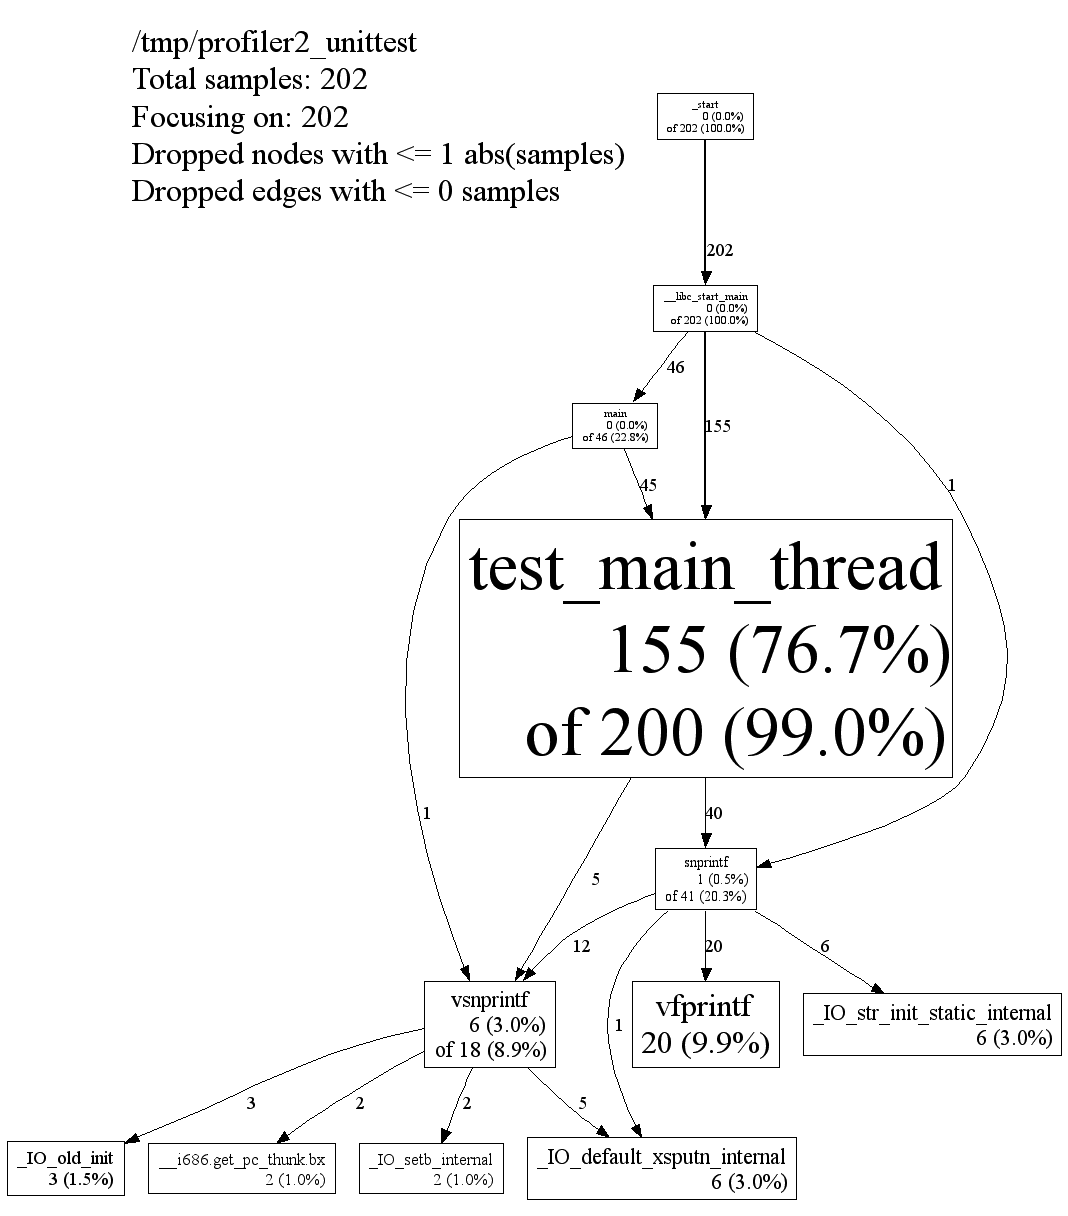
\includegraphics[scale=0.3]{images/pprof-test-big.png}
\end{center}

This shows the same numbers as the text output. Although this particular graphical example is on a different program than the text output, and that's why they look different. Directed edges denote function calls.
Note: 
\begin{center}
\# of samples in callees = \# in ``this function + callees'' - \# in ``this function''.
\end{center}

For example, in {\tt float\_math\_helper}, we have ``51 (local) of 96 (cumulative)''.
Here,
\[ 96 - 51 = 45 \mbox{(callees)}. \]
      \begin{itemize}
        \item callee {\tt int\_power} = 7 (bogus)
        \item callee {\tt float\_power} = 38
        \item callees total = 45
      \end{itemize}

Note that the call graph is not exact.
In fact, it shows many bogus relations which clearly don't exist.
For instance, we know that there are no cross-calls between {\tt int} and {\tt float} functions.

As with {\tt gprof}, optimizations will change the
      graph.\

You'll probably want to look at the text profile first, then use the
      {\tt --focus} flag to look at individual functions.

      \section*{System-level profiling}
Most profiling tools interrogate the CPU in more detail than {\tt
  gprof} and friends. These tools are typically aware of the whole
system, but may focus on one application, and may have both
per-process and system-wide modes. We'll discuss a couple of these
tools here, highlighting conceptual differences between these
applications.

\paragraph{Solaris Studio Performance Analyzer.} This 
tool\footnote{You can find a high-level description at
  \url{http://www.oracle.com/technetwork/server-storage/solarisstudio/documentation/oss-performance-tools-183986.pdf}}
supports {\tt gprof}-style profiling (``clock-based profiling'') as
well as kernel-level profiling through DTrace (described later). At
process level, it collects more process-level data than {\tt gprof},
including page fault times and wait times. It also can read CPU
performance counters (e.g. the number of executed floating point adds
and multiplies).  As a Sun application, it also works with Java
programs.

Since locks and concurrency are important, modern tools, including the
Studio Performance Analyzer, can track the amount of time spent
waiting for locks, as well as statistics about MPI message
passing. More on lock waits below, when we talk about WAIT.

\paragraph{VTune.} Intel and AMD both provide profiling
tools; Intel's VTune tool costs money, while AMD's CodeAnalyst tool is
free software.

Intel uses the term ``event-based sampling'' to refer to sampling 
which fires after a certain number of CPU events occur, and ``time-based
sampling'' to refer to the {\tt gprof}-style sampling (e.g. every 100ms).
VTune can also correlate the behaviour of the counters with other
system events (like disk workload). Both of these sampling modes
also include the behaviour of the operating system and I/O in their
counts.

VTune also supports an instrumentation-based profiling approach,
which measures time spent in each procedure (same type of
data as {\tt gprof}, but using a different collection scheme).

VTune will also tell you what it thinks the top problems with your
software are. However, if you want to understand what it's saying,
you do actually need to understand the architecture.

\paragraph{CodeAnalyst.} AMD also provides a profiling tool. Unlike Intel's tool, AMD's tool is
free software (the Linux version is released under the GPL), so that,
for instance, Mozilla suggests that people include CodeAnalyst
profiling data when reporting Firefox performance
problems~\footnote{\url{https://developer.mozilla.org/Profiling_with_AMD_CodeAnalyst}}.

CodeAnalyst is a system-wide profiler. It supports drilling down into
particular programs and libraries; the only disadvantage of being
system-wide is that the process you're interested in has to execute
often enough to show up in the profile. It also uses debug symbols to
provide meaningful names; these symbols are potentially supplied over
the Internet.

Like all profilers, it includes a sampling mode, which it calls ``Time-based
profiling'' (TBP). This mode works on all processors. The other modes are 
``Event-based profiling'' (EBP) and ``Instruction-based sampling'' (IBS);
these modes use hardware performance counters.

AMD's CodeAnalyst documentation points out that your sampling interval
needs to be sufficiently high to capture useful data, and that you need to 
take samples for enough time. The default sampling rate is once every
millisecond, and they suggest that programs should run for at least 15 seconds
to get meaningful data.

The EBP mode works like VTune's event-based sampling: after a certain
number of CPU events occur, the profiler records the system state.
That way, it knows where e.g. all the cache misses are occuring.
A caveat, though, is that EBP can't exactly identify the guilty statement,
because of ``skid'': in the presence of out-of-order execution, guilt
gets spread to the adjacent instructions.

To improve the accuracy of the profile information, CodeAnalyst uses
AMD hardware features to watch specific x86 instructions and ``ops'',
their associated backend instructions. This is the IBS mode\footnote{Available
on AMD processors as of the K10 family---typically manufactured in 2007+; see \url{http://developer.amd.com/assets/AMD_IBS_paper_EN.pdf}. Thanks to Jonathan Thomas for pointing this out.} of
CodeAnalyst.  AMD provides an
example\footnote{\url{http://developer.amd.com/cpu/CodeAnalyst/assets/ISPASS2010_IBS_CA_abstract.pdf}}
where IBS tracks down the exact instruction responsible for data
translation lookaside buffer (DTLB) misses, while EBP indicates four
potential guilty instructions.


\paragraph{oprofile.} This free software is a sampling-based tool which uses the Linux Kernel Performance
Events API to access CPU performance counters. It tracks the
currently-running function (or even the line of code) and can, in
system-wide mode, work across processes, recording data for every
active application.

Webpage: \url{http://oprofile.sourceforge.net}.

You can run oprofile either in system-wide mode (as root) or per-process. To run it in system-wide mode:
  \begin{lstlisting}
% sudo opcontrol --vmlinux=/usr/src/linux-3.2.7-1-ARCH/vmlinux
% echo 0 | sudo tee /proc/sys/kernel/nmi_watchdog
% sudo opcontrol --start
Using default event: CPU_CLK_UNHALTED:100000:0:1:1
Using 2.6+ OProfile kernel interface.
Reading module info.
Using log file /var/lib/oprofile/samples/oprofiled.log
Daemon started.
Profiler running.
  \end{lstlisting}

Or, per-process:
\begin{lstlisting}
[plam@lynch nm-morph]$ operf ./test_harness
operf: Profiler started

Profiling done.
\end{lstlisting}%$

Both of these invocations produce profiling output. You can read the profiling output
by running {\tt opreport} and giving it your executable.

  \begin{lstlisting}
% sudo opreport -l ./test    
CPU: Intel Core/i7, speed 1595.78 MHz (estimated)
Counted CPU_CLK_UNHALTED events (Clock cycles when not
halted) with a unit mask of 0x00 (No unit mask) count 100000
samples  %        symbol name
7550     26.0749  int_math_helper
5982     20.6596  int_power
5859     20.2348  float_power
3605     12.4504  float_math
3198     11.0447  int_math
2601      8.9829  float_math_helper
160       0.5526  main
  \end{lstlisting}
  If you have debug symbols ({\tt -g}) you can also get better data:
  {\small
  \begin{lstlisting}
% sudo opannotate --source --output-dir=/path/to/annotated-source /path/to/mybinary
  \end{lstlisting}
  }

Use {\tt opreport} by itself for a whole-system view.
    You can also reset and stop the profiling.
  \begin{lstlisting}
% sudo opcontrol --reset 
Signalling daemon... done
% sudo opcontrol --stop
Stopping profiling.
  \end{lstlisting}

\paragraph{perf.} This uses the same base data as oprofile, but provides a better
(git-like) interface. Once again, it is an interface to the Linux kernel's built-in
sample-based profiling using CPU counters. It works per-process, per-CPU, or system-wide.
It can report the cost of each line of code.

Webpage: \url{https://perf.wiki.kernel.org/index.php/Tutorial}

\noindent
Here's a usage example on some old assignment code from last year:
\begin{lstlisting}[basicstyle=\scriptsize]
[plam@lynch nm-morph]$ perf stat ./test_harness

 Performance counter stats for './test_harness':

       6562.501429 task-clock                #    0.997 CPUs utilized          
               666 context-switches          #    0.101 K/sec                  
                 0 cpu-migrations            #    0.000 K/sec                  
             3,791 page-faults               #    0.578 K/sec                  
    24,874,267,078 cycles                    #    3.790 GHz                     [83.32%]
    12,565,457,337 stalled-cycles-frontend   #   50.52% frontend cycles idle    [83.31%]
     5,874,853,028 stalled-cycles-backend    #   23.62% backend  cycles idle    [66.63%]
    33,787,408,650 instructions              #    1.36  insns per cycle        
                                             #    0.37  stalled cycles per insn [83.32%]
     5,271,501,213 branches                  #  803.276 M/sec                   [83.38%]
       155,568,356 branch-misses             #    2.95% of all branches         [83.36%]

       6.580225847 seconds time elapsed
\end{lstlisting} %$

\noindent
perf can tell you which instructions are taking time, or which lines
of code; compile with {\tt -ggdb} to enable source code viewing.

\begin{lstlisting}
% perf record ./test_harness
% perf annotate
\end{lstlisting}

\noindent
{\tt perf annotate} is interactive. Play around with it.

\paragraph{DTrace.} 
DTrace~\cite{Cantrill:2004:DIP:1247415.1247417} is an instrumentation-based
system-wide profiling tool designed to be used on production
systems. It supports custom queries about system behaviour: when you
are debugging system performance, you can collect all sorts of data
about what the system is doing. The two primary design goals were in
support of use in production: 1) avoid overhead when not tracing and
2) guarantee safety (i.e. DTrace can never cause crashes).

DTrace runs on Solaris and some BSDs. There is a Linux port, which may be usable.
I'll try to install it on {\tt ece459-1}.

\paragraph{Probe effect.} ``Wait! Don't `instrumentation-based' 
and `production systems' not go together?'' For instance, Valgrind incurs a 100$\times$
slowdown. Ouch.

Nope! DTrace was designed to have zero overhead when inactive. It does
this by dynamically rewriting the code to insert instrumentation when
requested. So, if you want to instrument all calls to the {\tt open}
system call, then DTrace is going to replace the instruction at the
beginning of {\tt open} with an unconditional branch to the
instrumentation code, execute the profiling code, then return to your
code. Otherwise, the code runs exactly as if you weren't looking.

\paragraph{Safety.} As I've mentioned before, crashing a production
system is a big no-no. DTrace is therefore designed to never cause a
system crash. How? The instrumentation you write for DTrace 
must conform to fairly strict constraints.

\paragraph{DTrace system design.} The DTrace framework supports instrumentation
\emph{providers}, which make \emph{probes} (i.e.  instrumentation
points) available; and \emph{consumers}, which enable probes as
appropriate. Examples of probes include system calls, arbitrary kernel
functions, and locking actions. Typically, probes apply at function entry or exit points.
DTrace also supports typical
sampling-based profiling in the form of timer-based probes; that is,
it executes instrumentation every 100ms. This is tantamount to
sampling.

You can specify a DTrace clause using probes, predicates, and a set of
action statements. The action statements execute when the condition
specified by the probe holds and the predicate evaluates to true. D
programs consist of a sequence of clauses.

\paragraph{Example.} Here's an example of a DTrace query from~\cite{Cantrill:2004:DIP:1247415.1247417}.

{ \begin{verbatim}
    syscall::read:entry {
            self->t = timestamp;
    }

    syscall::read:return
    /self->t/ {
            printf("%d/%d spent %d nsecs in read\n"
                pid, tid, timestamp - self->t);
    }
    \end{verbatim}
}

The first clause instruments all entries to the system call {\tt read}
and sets a thread-local variable {\tt t} to the current time. The
second clause instruments returns from {\tt read} where the
thread-local variable {\tt t} is non-zero, calling {\tt printf} to print out
the relevant data.

The D (DTrace clause language) design ensures that clauses cannot loop indefinitely
(since they can't loop at all), nor can they execute unsafe code;
providers are responsible for providing safety guarantees. Probes
might be unsafe because they might interrupt the system at a critical
time. Or, action statements could perform illegal writes. DTrace won't 
execute unsafe code.

\paragraph{Workflow.} Both the USENIX article~\cite{Cantrill:2004:DIP:1247415.1247417} and the
ACM Queue article~\cite{300ps} referenced above contain example usages of DTrace.
In high-level terms: first identify a problem; then, use
standard system monitoring tools, plus custom DTrace queries,
to collect data about the problem (and resolve it).

\section*{WAIT}
Another approach which recently appeared in the research literature is
the WAIT tool out of IBM. Unfortunately, this tool is not free and not
generally available. Let's talk about it anyways.

Like DTrace, WAIT is suitable for use in production environments. It
uses hooks built into modern Java Virtual Machines (JVMs) to analyze
their idle time. It performs a sampling-based analysis of the
behaviour of the Java VM. Note that its samples are quite infrequent;
they suggest that taking samples once or twice a minute is enough.  At
each sample, WAIT records the state of each of the threads, which
includes its call stack and participation in system locks. This data
enables WAIT to compute (using expert rules) an abstract ``wait
state''.  The wait state indicates what the process is currently doing
or waiting on, e.g. ``disk'', ``GC'', ``network'', or ``blocked''.

\paragraph{Workflow.} You run your application, collect data (using a
script or manually), and upload the data to the server. The server provides
a report which you use to fix the performance problems.
The report indicates processor utilization (idle, your application, GC, 
etc); runnable threads; waiting threads (and why they are waiting); 
thread states; and a stack viewer.

The paper presents six case studies where WAIT helped solve performance
problems, including deadlocks, server underloads, memory leaks, database
bottlenecks, and excess filesystem activity.

\subsection*{Other Applications of Profiling.} 
Profiling applies to languages beyond C/C++ and Java, of course. If you are
profiling an interpreted language, you'll need a specific tool to get useful
results. For Python, you can use {\tt cProfile}; it is a standard implementation
of profiling, from what I can see.


Here's a short tangent. Many of the concepts that we've seen for code
also apply to web pages. Google's Page Speed
tool\footnote{\url{http://code.google.com/speed/page-speed/}}, in
conjunction with Firebug, helps profile web pages, and provides
suggestions on how to make your web pages faster. Note that Page Speed
includes improvements for the web page's design, e.g. not requiring
multiple DNS lookups; leveraging browser caching; or combining images;
as well as traditional profiling for the JavaScript on your pages.


\bibliographystyle{alphaurl}
\bibliography{459}


\end{document}
